% \chapter{基于元学习本体增强的跨设备知识图谱表示模型}
% 本章将详细介绍提出的基于元学习本体增强的跨领域知识图谱表示学习模型的各个部分。本章首节对模型要解决的问题和测试的任务作出符号上的定义和解释;然后将介绍本文设计模型的整体框架以及对框架组成进行大概的描述;然后详细说明该知识表示模型的三个主要组成模块:关系编码模块、实体编码模块以及模型整体元学习训练设定与训练流程。此外对于训练集中可见的关系和实体,本文采用了传统的知识图谱表示学习的学习流程,即分别设置关系特征矩阵和实体特征矩阵,在初始化阶段对这两个矩阵按照各自目标维度随机赋值,在模型训练过程中通过TransE等打分函数对特征进行打分后进行更新,可以得到可见组件的特征嵌入。本章主要讲解本未见的组件进行编码的过程。该模型的主要创新点如下:(1)关系和实体的表示能够同时学习到实体三元组结构上的拓扑信息和本体层面上的语义信息。(2)能够通过元学习的训练流程模拟出目标问题的学习任务对模型参数进行更新。(3)能够同时对测试集中未见的关系和未见的实体嵌入编码。
% \section{问题定义}
% 一个单独的知识图谱通常定义为\(\mathcal{G} = (\mathcal{E},\mathcal{R},\mathcal{T})\),其中\(\mathcal{E}\)指代所有图谱实体的集合,\(\mathcal{R}\)指代图谱所有关系的集合而\(\mathcal{T}\)指代所有的实体三元组,而且对于三元组集合\(\mathcal{T}=\{(h,r,t) \subseteq \mathcal{E} \times \mathcal{R} \times \mathcal{E}\}\),即所有的三元组的头尾实体和关系均来自于实体集\(\mathcal{E}\)和关系集\(\mathcal{R}\)中。对于知识图谱上的链接预测任务,则是给定一个三元组的头结点和关系\((h,r,?)\)或者尾结点和关系\((?,r,t)\)来预测缺失的实体节点\(e \in \mathcal{E}\),使得该缺失的实体节点能构成一个事实三元组\((h,r,t)\)来完成对原始知识图谱的知识补全。为了评估表示学习模型在链接预测任务上的效果,通常会设置两组三元组数据,一组训练三元组\(\mathcal{T}_{support}\)用于对表示学习模型的参数进行学习,另一组测试三元组\(\mathcal{T}_{query}\)包含了训练集中不存在的知识图谱的其他隐藏的事实三元组用于对模型的学习效果进行测试。例如对一个尾结点的预测任务,给定在测试三元组中的一个事实\((h,r,t) \in \mathcal{T}_{query}\),通过模型计算所有可能预测三元组\(\{(h,r,e) | e \in \mathcal{E}, (h,r,e) \notin \mathcal{T}_{support} \cup \mathcal{T}_{query}\}\),如果在所有预测三元组中\((h,r,t)\)的得分越高则说明该表示模型的效果越好。

% 而在跨设备的训练场景下,本文对传统的知识图谱链接预测任务的定义进行了场景适配。现给定一个基础的训练知识图谱\(\mathcal{G}^{train} = (\mathcal{E}^{train},\mathcal{R}^{train},\mathcal{T}^{train})\),训练的目标是在训练知识图谱上进行模型参数的学习,从而能够将该模型应用在包含未见组件的新兴测试知识图谱上,即\(\mathcal{G}^{test} = (\mathcal{E}^{test},\mathcal{R}^{test},\mathcal{T}^{test}_{support},\mathcal{T}^{test}_{query})\),其中的实体集和关系集遵循\((\mathcal{E}^{train} \neq \mathcal{E}^{test},\mathcal{E}^{train} \cap \mathcal{E}^{test} \neq \emptyset)\)及\((\mathcal{R}^{train} \neq \mathcal{R}^{test},\mathcal{R}^{train} \cap \mathcal{R}^{test} \neq \emptyset)\)。其中只用于标记测试集中实体与关系的结构,不用于对模型的训练。而且在跨设备的设定下,测试数据集和训练数据集无法进行数据合并。
% \section{模型整体架构}
% % \begin{figure}[h]
% %   \centering
% %   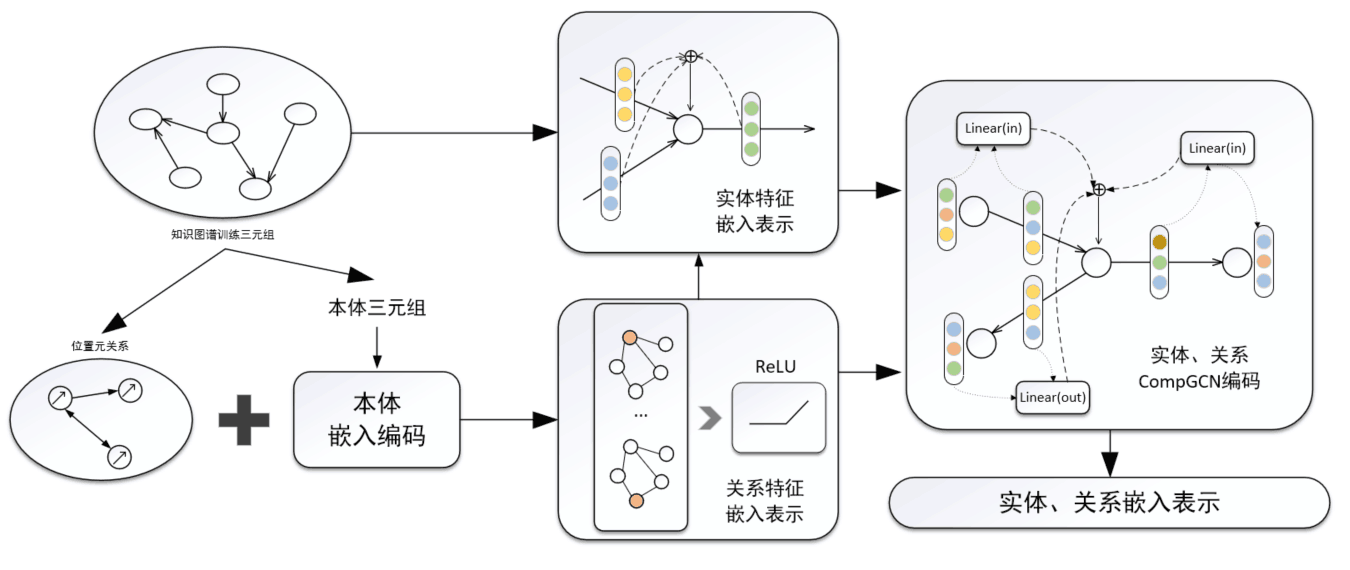
\includegraphics[width=1\textwidth]{3-1.png}
% %   \caption{模型架构图}
% %   \label{fig:3-1}
% % \end{figure}
% 本文提出的模型整体结构图如图\ref{fig:3-1}所示,总体包含三个大的模块:关系编码模块、实体编码模块、实体关系联合嵌入模块。

% 为了对关系的特征进行提取,本文模型首先根据实例图谱中的关系的相对位置结构构建出关系位置图,该图中的节点为实例图谱中的关系。然后基于图谱的本体三元组信息对本体的关系及概念节点进行嵌入,为了补充本体的信息,同时采用概念节点的描述文本对本体嵌入进行加强;然后将本体信息和关系位置图进行结合,通过两层GCN模型对关系的语义信息和结构信息进行更新和学习,获得关系特征的嵌入表示。对实体的表示上,通过聚合实体邻接关系,通过学习关系方向调整矩阵的参数来对所有关系的特征进行提取获得实体特征的嵌入表示。最后为了加强实体与关系的联系,本文模型在实例图谱上进行两层CompGCN的特征提取获得了最终的实体和关系的嵌入,同时修改了CompGCN的输出层使得关系和实体的维度不要求一致,从而可以通过多种KGE模型作为打分函数计算损失函数对模型调优。

% 其中对本体嵌入的过程中,本文首先从基础的三元组数据中学习到结构化的嵌入表示,然后从三元组的概念节点的描述信息中使用词嵌入学习到概念节点的描述文本嵌入,为了将描述文本的嵌入补充到本体信息的结构化中去,本文使用一个共享参数的线性层将结构化嵌入表示和描述文本嵌入表示映射到同一个表示空间中。在映射后的线性层中,参照TransE的评分思想,本文采用三个距离打分函数将映射后的两种嵌入表示联合更新,学习到兼顾结构信息和描述文本信息的嵌入表示。最后将两种表示拼接作为本体信息进行后续操作。本体嵌入整体结构图如下:
% % \begin{figure}[h]
% %   \centering
% %   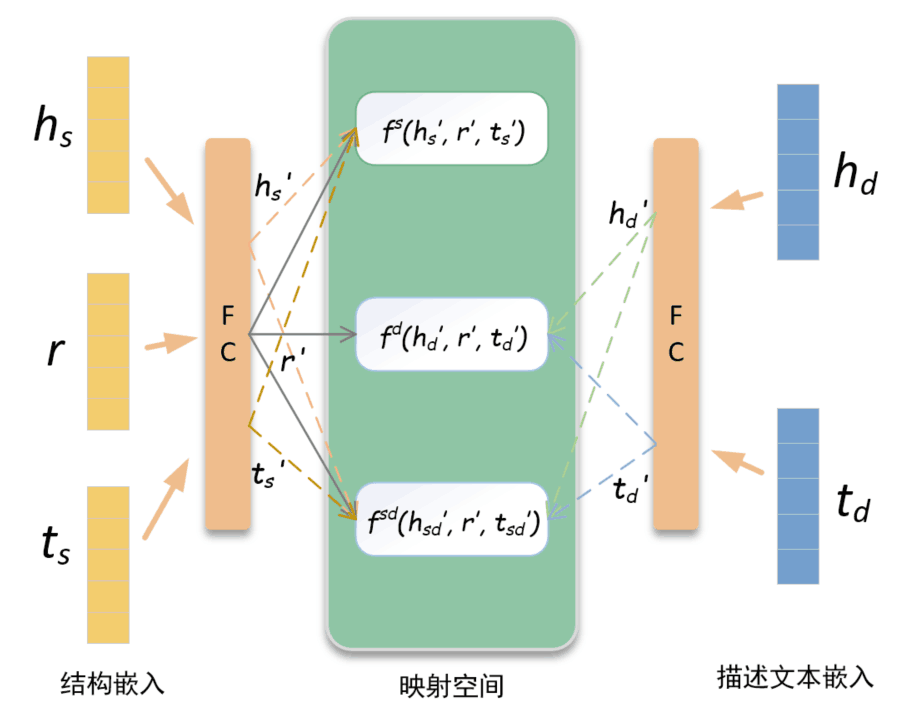
\includegraphics[width=0.9\textwidth]{3-2.png}
% %   \caption{本体嵌入架构}
% %   \label{fig:3-2}
% % \end{figure}

% \section{关系嵌入模块}
% \subsection{本体信息嵌入}
% 为了能从本体三元组的结构数据中捕捉到能够辅助实体三元组编码,特别是包含未见组件的本体概念信息,本文首先需要将本体三元组转换为响应的语义信息编码。与传统的知识图谱嵌入表示类似,对于一个本体三元组\((c_{i},p,c_{j})\),本体语义信息编码的目的就是设计出一个打分函数\(f(c_{i},p,c_{j})\)作为编码模型的激活函数,本文分别采用了传统的知识图谱嵌入方法如TransE对本体三元组进行编码,然后将编码后的本体信息用于辅助关系编码。例如按照TransE模型的设定,本体三元组的元关系属性是头尾两个实体节点的转移量,将打分函数设置为:
% \begin{equation}
%   f_{TransE}(c_{i},p,c_{j}) = - \| \textbf{c}_{i} + \textbf{p} + \textbf{c}_{j}\| \label{eq:3-1}
% \end{equation}

% 其中\(\textbf{c}_{i}\),\(\textbf{p}\),\(\textbf{c}_{j}\),是一个本体三元组响应的概念编码和元关系编码。同时为了提高所有本体三元组的嵌入效果,本文采用自对抗负抽样损失函数来对计算损失更新模型:
% \begin{equation}
%   \mathcal{L}_{\mathcal{O}} = \frac{1}{\mid \mathcal{T}_{\mathcal{O}}\mid} \sum_{(c_{i},p,c_{j}) \in \mathcal{T}_{\mathcal{O}}} [\gamma _{o} + f(c'_{i},p,c'_{j}) + f(c_{i},p,c_{j})] \label{eq:3-2}
% \end{equation}

% 公式中\(\gamma _{o}\)是控制正负样本得分的参数,同时\(c'_{i}\),\(c'_{j}\)是不存在与本体三元组中的负样本,为了生成这些负样本,本文在所有的本体概念中分别遮盖住已存在的本体三元组的头节点和尾结点,然后从所有本体节点中随机筛选出其他节点组成负样本。
% 本体信息除了结构化的本体三元组之外,还有许多对本体的详细描述文本,如本体节点“companyceo”的描述文本“specifies that a particular CEO is the CEO of a particular company”。这些描述文本可以在对本体信息提取的时候提供额外的语义信息,因此本文通过文本描述进一步加强了对本体三元组的语义嵌入。但是描述文本的建模和一般的三元组建模因为模型的差异一定无法直接进行融合,因此对于一个特定的本体三元组\((c_{i},p,c_{j})\),本文首先获得了三元组结构的嵌入\(h_{s}/r/t_{s} \in \mathbb{R}^{d_{1}}\)以及对每一个本体节点描述文本的向量表示\(h_{d}/t_{d} \in \mathbb{R}^{d_{2}}\)来指代文本描述信息,为了能够让这两个不同层面的嵌入进行融合,本文引入一个全连接层将两个不同的嵌入同时映射到同一个表示维度上,映射后的结构嵌入和文本嵌入分别表示为\(h_{s}^{'}\)和\(h_{d}^{'}\),在统一后的表示空间中使用TransE对三元组结构的嵌入进行打分:
% \begin{equation}
%   f^{s} = -  \parallel h'_{s} + r' - t'_{s}  \parallel \label{eq:3-3}
% \end{equation}

% 对描述文本的嵌入进行打分:
% \begin{equation}
%   f^{d} = -  \parallel h'_{d} + r' - t'_{d}  \parallel \label{eq:3-4}
% \end{equation}

% 同时为了为了使这两种类型的表示相互兼容和互补,本文遵循DKRL模型的设定来定义交叉和相加得分函数:
% \begin{equation}
%   f^{sd} = -  \parallel h'_{s} + r' - t'_{d}  \parallel -  \parallel h'_{d} + r' - t'_{s}  \parallel \label{eq:3-5}
% \end{equation}

% 所有的四个得分函数综合可以保证两个层面的嵌入表示可以在相同空间里进行学习和更新,最后本体嵌入的得分函数表示为:
% \begin{equation}
%   f^{sd} = -  \parallel h'_{s} + r' - t'_{d}  \parallel -  \parallel h'_{d} + r' - t'_{s}  \parallel \label{eq:3-6}
% \end{equation}

% 因此在本体嵌入的损失函数也响应的转化为:
% \begin{equation}
%   \mathcal{L}_{\mathcal{O}}^{ont} = \frac{1}{\mid \mathcal{T}_{\mathcal{O}}\mid} \sum_{(c_{i},p,c_{j}) \in \mathcal{T}_{\mathcal{O}}} [\gamma _{o} + f'(c'_{i},p,c'_{j}) + f'(c_{i},p,c_{j})] \label{eq:3-7}
% \end{equation}

% 经过训练后每个本体节点都有两个层面的嵌入:三元组结构嵌入和描述文本嵌入,然后本文将这两种映射后的嵌入进行拼接作为本体节点的最终的向量表示。上述的描述文本的向量表示,本文采用了CNN网络进行生成。

% \subsection{关系图构建}
% 对未见的关系,由于在训练集中没有相关的三元组可以提供特征学习的支持,所以必须要从除三元组以外的其他层面获取到可以对未见关系编码的特征表示。而关系作为构成知识图谱的一种结构信息,关系受相连节点的影响会与其他关系存在联系,这些联系可以作为关系的一种拓扑特征信息,类似的研究也有使用节点的度作为节点特征进行学习的尝试。这些结构性的信息会减少对训练集数据的依赖,在对关系特征进行学习的时候可以通过聚合相连其他关系的信息来对关系进行特征表示,能够较好作用在未见的关系上。

% 为了对关系的结构特征进行学习,本文继承了TACT模型对于关系的拓扑设定,将相邻的两个关系按照关系的方向抽取出四种元关系类型,并将关系视为节点,关系与关系之间由元关系进行连接。
% % \begin{figure}[h]
% %   \centering
% %   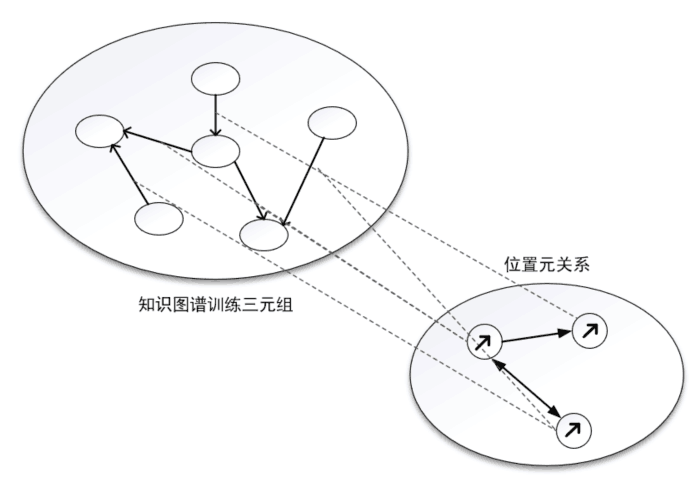
\includegraphics[width=0.5\textwidth]{3-3.png}
% %   \caption{从实体关系构建关系图}
% %   \label{fig:3-3}
% % \end{figure}

% 这些元关系根据关系的相对关系设置为四类,如图\ref{fig:3-4}所示,分别为tail-head、head-tail、tail-tail、head-head。元关系的head和tail都代表了两个相邻关系的指向,比如(relation1,tail-head,relation2)代表同一个实体连接的两个相邻关系1和关系2,且关系1指向该实体而关系2则从该实体指向其他实体。对于在训练三元组中的两个关系,如果它们符合其中一种的相对未见关系,则在关系位置图中创建一个关系结点,并通过与关系进行连接。
% % \begin{figure}[h]
% %   \centering
% %   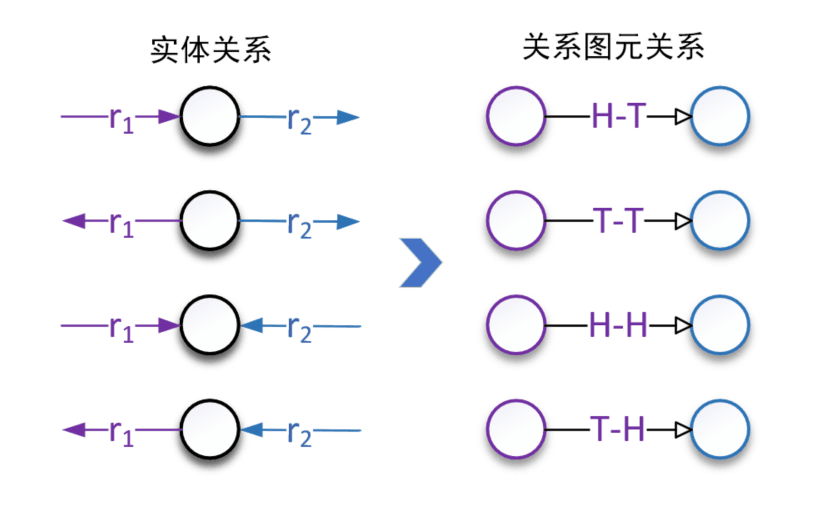
\includegraphics[width=0.5\textwidth]{3-4.png}
% %   \caption{实体关系与关系图元关系的映射}
% %   \label{fig:3-4}
% % \end{figure}

% 因此根据输入的实体三元组,可以将原始的图结构转变为关系相关图,同时在构建图的过程中没有使用到任何额外的实体属性或关系属性,可以作用到任何未见或已知的关系上。在关系相关图中的节点代表关系,边表示在原始三元组任意两个关系对应的元关系。

% \subsection{关系相关性系数聚合编码}
% 在位置本体图中结点为原三元组中的关系,其位置结构部分的特征可以通过聚合关系结点的其他相邻关系结点的特征获取该关系的特征。为了能够将本体的嵌入作为对关系嵌入的语义补充,在构建好的关系位置图上本文通过对关系节点到本体概念的映射获取到各关系节点的初始化特征表示,然后通过多层GCN网络聚合邻接节点的特征来加强对关系节点的特征学习,对于节点的更新公式如下:
% \begin{equation}
%   h_{v} = f\left( \sum_{(u,r) \in \mathcal{N}(v)} W h_{u}\right) \label{eq:3-8}
% \end{equation}

% 其中\(h_{u}\)是相邻关系节点的特征,每层GCN会有两步的操作,首先左乘归一化后的邻接矩阵对邻居节点的特征进行聚合,然后右乘一个可学习的线性转换矩阵\(W_{r}\)将输入的特征映射到目标特征空间中,最后使用一个非线性的激活函数来获取本层的特征输出。

% 为了区分在链接预测任务中不同元关系的的重要性,本文在对不同元关系连接的关系特征进行聚合时设置一个可学习的权重参数,根据任务的表现来学习不同元关系对应的重要程度,计算公式转化为:
% \begin{equation}
%   h_{v} = f\left( \sum_{(u,r) \in \mathcal{N}(v)} W_{ \lambda(r) } h_{u}\right) \label{eq:3-9}
% \end{equation}

% 其中\(w_{r}\)是两个关系节点相连的元关系类型相对应的参数,根据本文设定的四种不同的元关系,该系数由四个不同的参数控制:
% \begin{equation}
%   W_{dir(r)} = \left\{ \begin{array}{rcl}
%     &W_{t-h}  \mbox{,} &\quad r \in R_{tail-head} \\
%     &W_{h-t}  \mbox{,} &\quad  r \in R_{head-tail} \\
%     &W_{t-t}  \mbox{,} &\quad  r \in R_{tail-tail} \\
%     &W_{h-h}  \mbox{,} &\quad  r \in R_{head-head} \\
%     \end{array}\right\} \label{eq:3-10}
% \end{equation}

% \section{实体嵌入模块}
% 对于未见的实体特征提取,本文认为对一个未见的实体可通过它连接的关系来进行预测。如图\ref{fig:3-5}所示,右侧未见实体X的关系结构和Tom的关系相似,可以推断出3是一个类似Tom的一个学生节点,所以本文通过聚合实体所有关系来对实体进行表示。
% \begin{figure}[h]
%   \centering
%   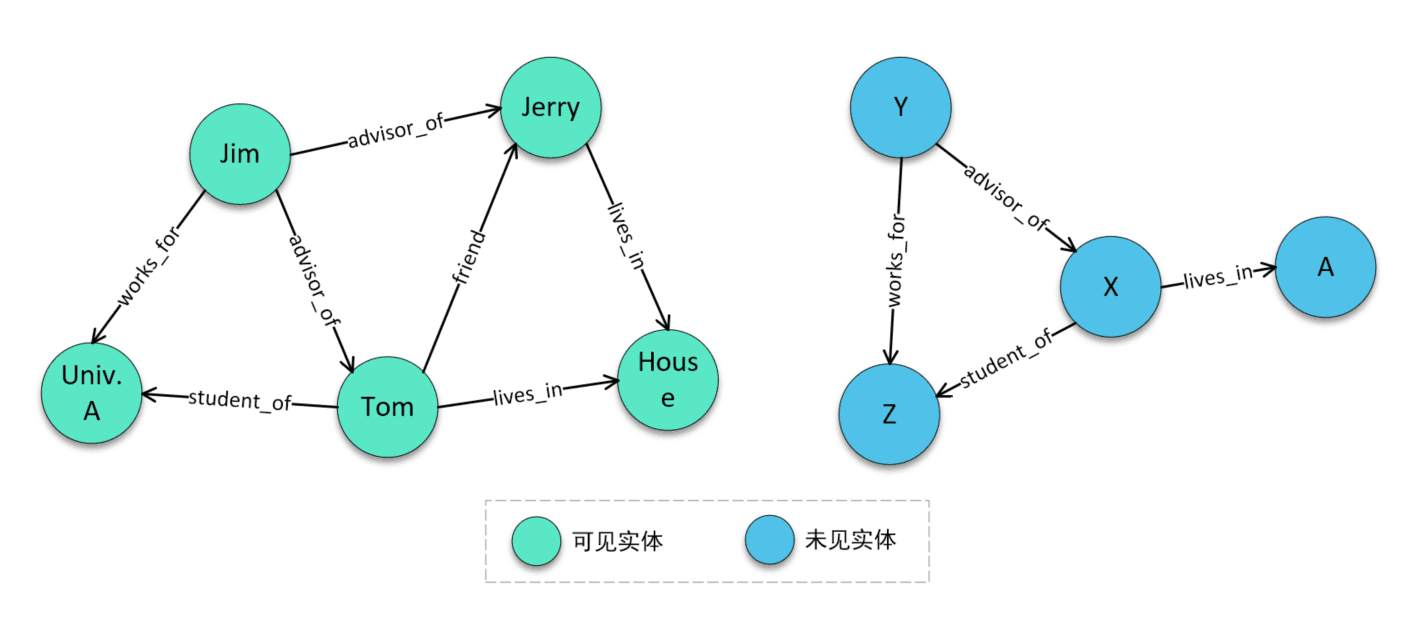
\includegraphics[width=0.8\textwidth]{3-5.png}
%   \caption{未见实体的关系特征}
%   \label{fig:3-5}
% \end{figure}

% 同时考虑到实体关系的方向性,本文通过以下公式来进行实体特征的聚合:
% \begin{equation}
%   h_{e} = \frac{1}{ \mid \mathcal{N}(e) \mid} \sum_{r\in\mathcal{N}(e)} W^{ent}_{dir(r) }h_{r} \label{eq:3-11}
% \end{equation}

% \(\mathcal{N}(e)\)是实体e所有连接关系的集合;\(W^{ent}_{dir(r)}\)是用于将关系特征转化为实体特征且区分方向的一个转换参数,\(W^{ent}_{dir(r)}\)在关系r为指向实体e时表示为\(W^{ent}_{in}\),当关系r由实体e指向其他实体时记作\(W^{ent}_{out}\)。

% \section{实体关系联合嵌入模块}
% 为了将关系特征聚合获得的实体特征进行抽取,本文在将输出的特征作为输入放到一个GNN网络中进行更新和编码得到学习后的嵌入,该GNN网络也以CompGCN模型为基础,但是将模型原有的实体关系聚合器修改为了一个线性转化层可以更好适应以多种传统KGE方法如RotatE来作为解码器进行下游任务,GNN层的实体嵌入更新如下:
% \begin{equation}
%   m _ { e } ^ { l + 1 } = \sum _ { ( r , t ) \in \mathcal{O} ( e ) } W _ { \text { out } } ^ { l } [ h _ { r } ^ { l } ; h _ { t } ^ { l } ] + \sum _ { ( r , h ) \in\mathcal{I} ( e ) } W _ { in } ^ { l } [ h _ { r } ^ { l } ; h _ { h } ^ { l } ]  \label{eq:3-12}
% \end{equation}

% \(\mathcal{O} ( e )\)是实体e的所有指向其他节点的关系和实体的集合,\(\mathcal{I} ( e )\)是所有指向其他节点e的关系和实体的集合,\( W _ { in } ^ { l }\)和\( W _ { out } ^ { l }\)分别是在GNN网络的第l层对实体的入关系和出关系的可学习的参数,\([;]\)而指代两个向量的连接操作。经由一层的GNN网络对特征的聚合后,实体的特征转换公式如下:
% \begin{equation}
%   h _ { e } ^ { l + 1 } = \sigma \left( \frac { m _ { e } ^ { l + 1 } } { | \mathcal{O} ( e ) | + | \mathcal{I} ( e ) | } + W _ { \text { self } } ^ { l } h _ { e } ^ { l } \right) \label{eq:3-13}
% \end{equation}

% \(W _ { \text { self } } ^ { l }\)是针对实体e本身特征自循环更新的模型学习参数,\(\sigma\)指代模型GNN模型的激活函数。同时,关系也在该层GCN中也进行了更新操作:
% \begin{equation}
%   h _ { r } ^ { l + 1 } = \sigma (W _ { \text { self } } ^ { l } h _ { r } ^ { l }) \label{eq:3-14}
% \end{equation}

% 经过两层GCN对关系嵌入和实体嵌入的更新,该GNN模块即可输出该训练任务下所有可见组件以及未见组件的知识提取表示,用于本次任务的loss的计算及模型参数更新。

% \section{元学习训练设定}
% 为了能够对知识图谱中的未见关系和未见实体进行表示学习,借鉴于元学习learning to learn的思想,本文从训练集中抽取了一系列包含未见实体和关系的训练任务来模拟测试环境,并且在该训练环境中对模型进行训练。

% 每个训练任务\(\mathcal{S}^{i} = (\mathcal{E}^{i}, \mathcal{R}^{i}, \mathcal{T}^{i}_{sup},\mathcal{T}^{i}_{que})\)包含训练实体集、关系集、support训练三元组集以及query测试三元组集。为了模拟未见的组件,将部分实体和关系标记为未见,每个训练任务被重新定义为如下:
% \begin{equation}
%   \mathcal{S}^{i} = (\mathcal{E}^{i} = (\hat{\mathcal{E}}^{i},\tilde{\mathcal{E}}^{i}), \mathcal{R}^{i} = (\hat{\mathcal{R}}^{i} ,\tilde{\mathcal{R}}^{i}   ), \mathcal{T}^{i}_{sup},\mathcal{T}^{i}_{que})  \label{eq:3-15}
% \end{equation}

% \(hat{\mathcal{E}}^{i} \in \mathcal{E}^{train}\)指代实体集中的可见实体而\(\tilde{\mathcal{E}}^{i} \notin \mathcal{E}^{train}\)指代未见的实体;\(\hat{\mathcal{R}}^{i} \in \mathcal{R}^{train}\)指代关系集中的可见关系\(\tilde{\mathcal{R}}^{i} \notin \mathcal{R}^{train}\)指代未见的关系。因此所有训练的总目标是基于每个任务的support集上进行对未见组件的训练使得在query集上的评估得分最高:
% \begin{equation}
%   \max\limits_{ \theta } \mathbb{E} _ { S ^ { i } \sim p ( S ) } \left[ \sum\limits_{ ( h , r , t ) \in \mathcal{T} _ { \text { que } } ^ { i } } \frac { 1 } { | \mathcal{T} _ { \text { que } } ^ { i } | } \mathcal{M} _ { \theta } ( h , r , t | \mathcal{T} _ { \text { sup } } ^ { i } ) \right] \label{eq:3-16}
% \end{equation}

% 其中\(\mathcal{M}\)可以通过在support集上学习到响应的模型参数然后在query集上对三语组进行可行性打分,结合前几节模型中学习到的两个分散的embedding对三元组进行打分。本文采用自对抗负抽样损失函数来对计算损失更新模型:
% \begin{equation}
% \begin{aligned}
%   \mathcal{L}(\mathcal{S}^{i}) = &\frac{1}{|\mathcal{T}^{i}_{que}|} \sum\limits_{(h,r,t)\in\mathcal{T}^{i}_{que}}-log\sigma(\gamma + s(h,r,t)) \\
%   &-\sum\limits_{i=1}^{n}p(h'_{i},r,t'_{i})log\sigma(-\gamma - s(h,r,t)) \label{eq:3-17}
% \end{aligned}
% \end{equation}

% n指代负采样的数量,\(p(h'_{i},r,t'_{i})\)指代负采样的权重系数,\(s(h,r,t)\)是用于计算embedding在query三元组上的得分函数。

% \section{链接预测任务及训练流程}
% 链接预测任务主要是基于知识图谱已有事实来推断出知识图谱中当前不存在的事实三元组,根据待预测节点的不同可区分为头结点预测和尾结点预测,通过比较测试的事实三元组在模型预测的事实三元组排名中出现的概率来评估模型链接预测任务的好坏。本文在进行每次任务损失的过程中,通过正负样本的联合计算出损失,并以此进行梯度下降求解。负样本损失计算公式如下:
% \begin{equation}
% \mathcal{L}_{neg} = \sum_{i = 1}^{n} \left( softmax(W[s_{tail};s_{head}])log \sigma (- [s_{tail};s_{head}]) \right) \label{eq:3-18}
% \end{equation}

% 其中\(s_{tail}\)和\(s_{head}\)是对一个测试三元组对应的尾结点负采样得分和头结点负采样得分,n代表负采样的数量,\([;]\)操作将正负样本的得分矩阵进行简单的连接操作,\(W\)是对得分进行微调的权重参数,本文默认设置为1。之后和正样本的得分求得算术平均即为该测试三元组的单个损失。

% 对于模型的训练流程,本文按照元学习单任务训练方法进行,每个任务的目标都是使该任务下的连接预测效果最优,具体流程如下:

% \begin{enumerate}[label=\arabic*)]
%   \item 初始化模型参数,主要包含了训练数据集中可见实体和关系的嵌入初始化、元关系的权重参数以及两个不同阶段的GCN层和CompGCN层的传递参数。
%   \item 获得任务的支持集和查询集,主要从原训练集中抽取单个任务的子图,并划分为支持集和查询集,同时对关系和节点的标签进行设置以模拟出未见组件。
%   \item 单次任务训练获得实体关系的嵌入,通过KGE模型计算查询集损失,通过损失函数进行梯度下降求解。
%   \item 更新模型参数,重复下一个任务的训练直至效果不再更优。
%   \item 对测试集进行模型测试,输出任务得分。
% \end{enumerate}

% \section{本章小结}
% 本章从本文模型的总体架构开始逐步详细介绍了模型的各个组成部分,包括主要的关系编码模块、实体编码模块以及元学习训练任务的定义和训练流程的说明。在关系编码模块说明了本文模型如何对关系的拓扑结构进行提取以及如何通过GCN层对关系的本体信息和拓扑信息进行融合学习,从而学习到未见关系的有效表示;在实体编码模块,通过未见实体的邻接关系的特征聚合进行表示,并且在实例知识图谱之上再次通过GNN来聚合其他关系和实体信息完成最后的特征表示。之后的章节中将对本文模型在测试数据集上进行充分的实验,检验本文模型的有效性。